\documentclass{standalone}
\usepackage{../../../../preamble_tikz}
\usepackage{../../../../preamble_math}

\begin{document}
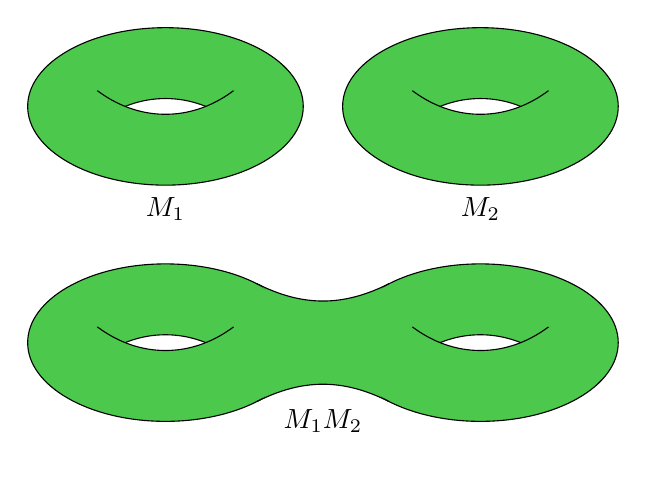
\begin{tikzpicture}
  \def\a{2}
  \def\b{0.5}
  \def\manifold#1#2#3#4{
    \draw[fill=#4] (#1,#2) ellipse (1.75 and 1);
    \begin{scope}
      \clip (#1,#2+2.2) ellipse (1.75 and 2.3);
      \draw[fill=white] (#1,#2-2.2) ellipse (1.75 and 2.3);
    \end{scope}
    \begin{scope}
      \clip (#1,#2-1.8) ellipse (1.75 and 2.3);
      \draw (#1,#2+2.2) ellipse (1.75 and 2.3);
    \end{scope}
    \node at (#1,-1.3+#2){#3};
  }
  \def\union#1#2{
    \fill[green!70!black!70]
    (#1+-0.8425,#2+0.75) to[out=-26.746,in=180+26.746]
    (#1+0.8425,#2+0.75) to[out=180+26.746,in=180-26.746]
    (#1+0.8425,#2+-0.75) to[out=180-26.746,in=26.746]
    (#1+-0.8425,#2+-0.75) to[out=26.746,in=-26.746]
    (#1+-0.8425,#2+0.75);
    \draw[black]
    (#1+-0.8425,#2+0.75) to[out=-26.746,in=180+26.746]
    (#1+0.8425,#2+0.75)
    (#1+0.8425,#2+-0.75) to[out=180-26.746,in=26.746]
    (#1+-0.8425,#2+-0.75);
  }
  \useasboundingbox (-\a-1.75,-1.4) rectangle (\a+1.75,4);
  %%% M1
  \manifold{-\a}{3}{$M_1$}{green!70!black!70}

  %%% M2
  \manifold{\a}{3}{$M_2$}{green!70!black!70}

  %%% M1+M2
  \manifold{-\a}{0}{}{green!70!black!70}
  \manifold{\a}{0}{}{green!70!black!70}
  \union{0}{0}

  \node at (0,-1){$M_1\conn M_2$};
\end{tikzpicture}

\end{document}